\makeatletter
\def\beamer@andtitle{\unskip,  }% Replace \and between author names (original definition is \quad), see https://tex.stackexchange.com/a/596731
\def\beamer@andinst{\\[1pt]}% See https://tex.stackexchange.com/a/201716
\makeatother

\maketitle
\section{Introduction}

\begin{frame}{Introduction}
\begin{columns}
\begin{column}{0.5 \textwidth}
    \begin{itemize}
        \item Thesis' aim: satellite docking, stabilization and inertia retrieval.
        \item Docking $\rightarrow$ \textit{impact}.
        \item Manipulator: robotic arm:
        \begin{itemize}
        \item Rigid bodies: \textit{links}
        \item Relative motion: \textit{joints}
        \item Actuation: \textit{motors}
        \end{itemize}
        \item Vehicle-Manipulator System: VMS.
    \end{itemize}
\end{column}
\begin{column}{0.5 \textwidth}
\begin{figure}
\centering
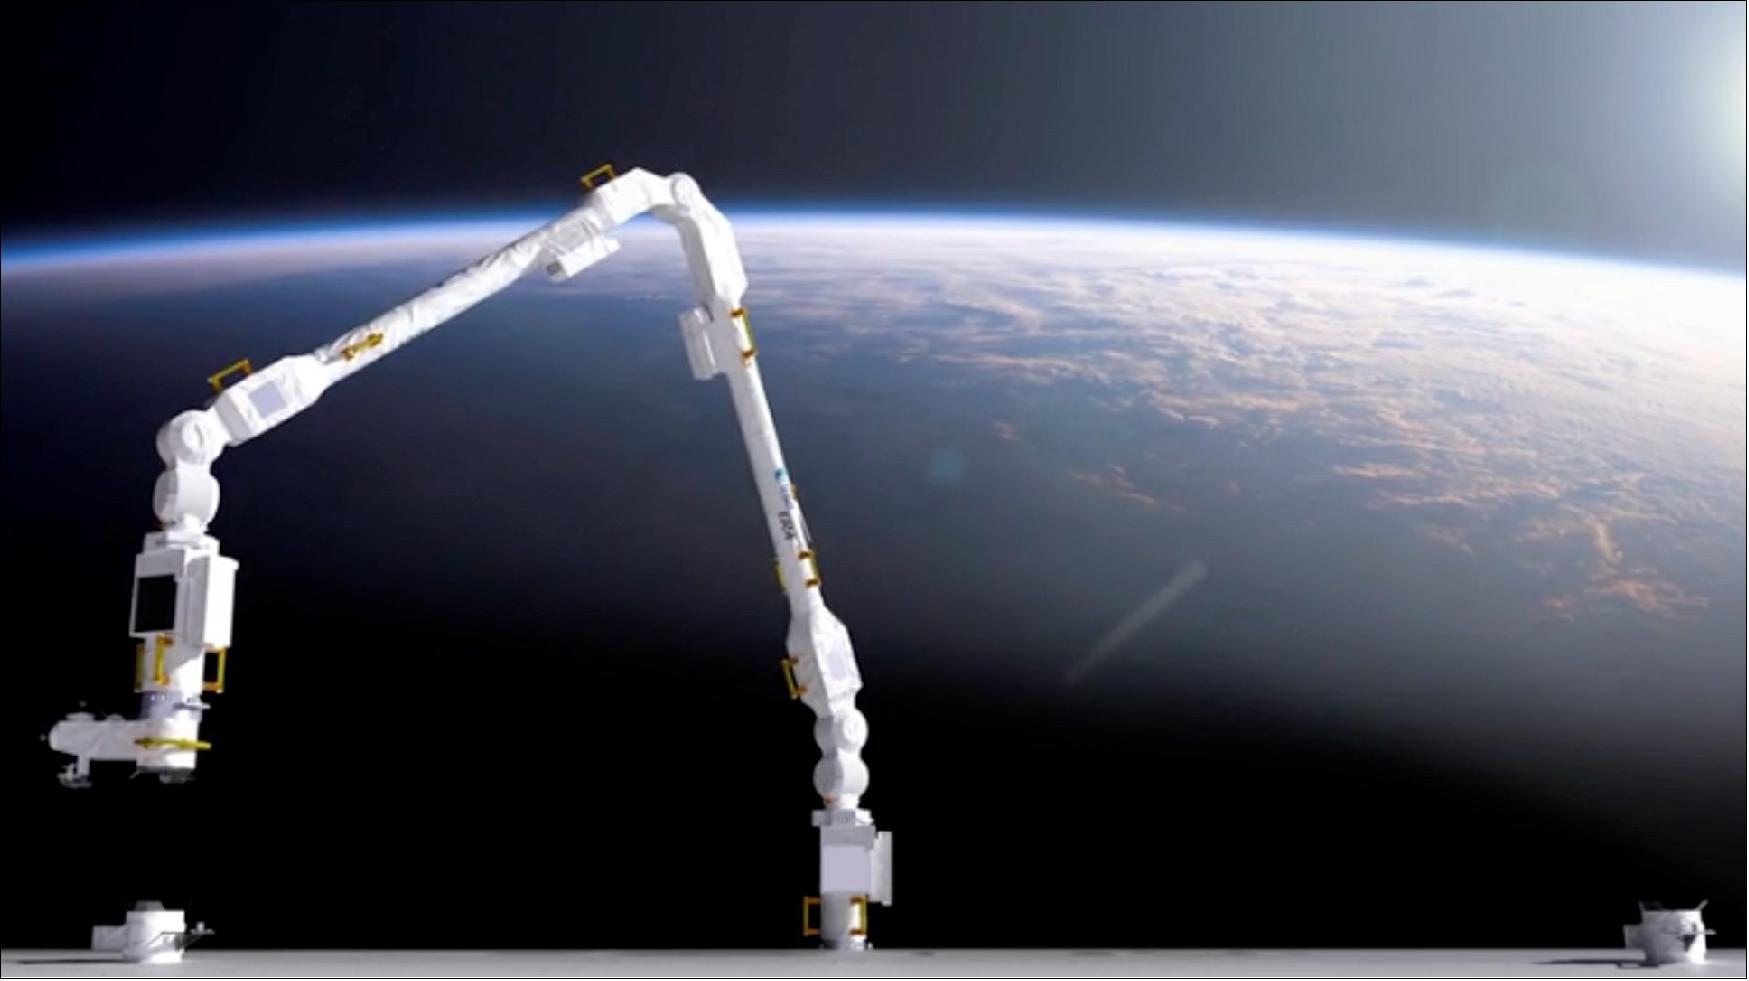
\includegraphics[scale=0.2]{era.jpeg}
\caption{ESA's space manipulator~\cite{esa}.}
\end{figure}
\end{column}
\end{columns}
\end{frame}

\section{Overview}

\begin{frame}{Historical Background}
\begin{columns}
\begin{column}{0.5 \textwidth}  
\begin{itemize}
    \item First space manipulator: Space Remote Manipulator System (SRMS), 11/1981 - 07/2011.
    \item First space mission: MIR, 1986 - 2001.
    \item Japanese arm: 2008.
    \item Canadarm2 (or SSRMS) and MSS: 04/2001
    \item ESA's manipulator, ERA: 07/2021
\end{itemize}
\end{column}
\begin{column}{0.5 \textwidth}  
    \begin{figure}
        \centering
        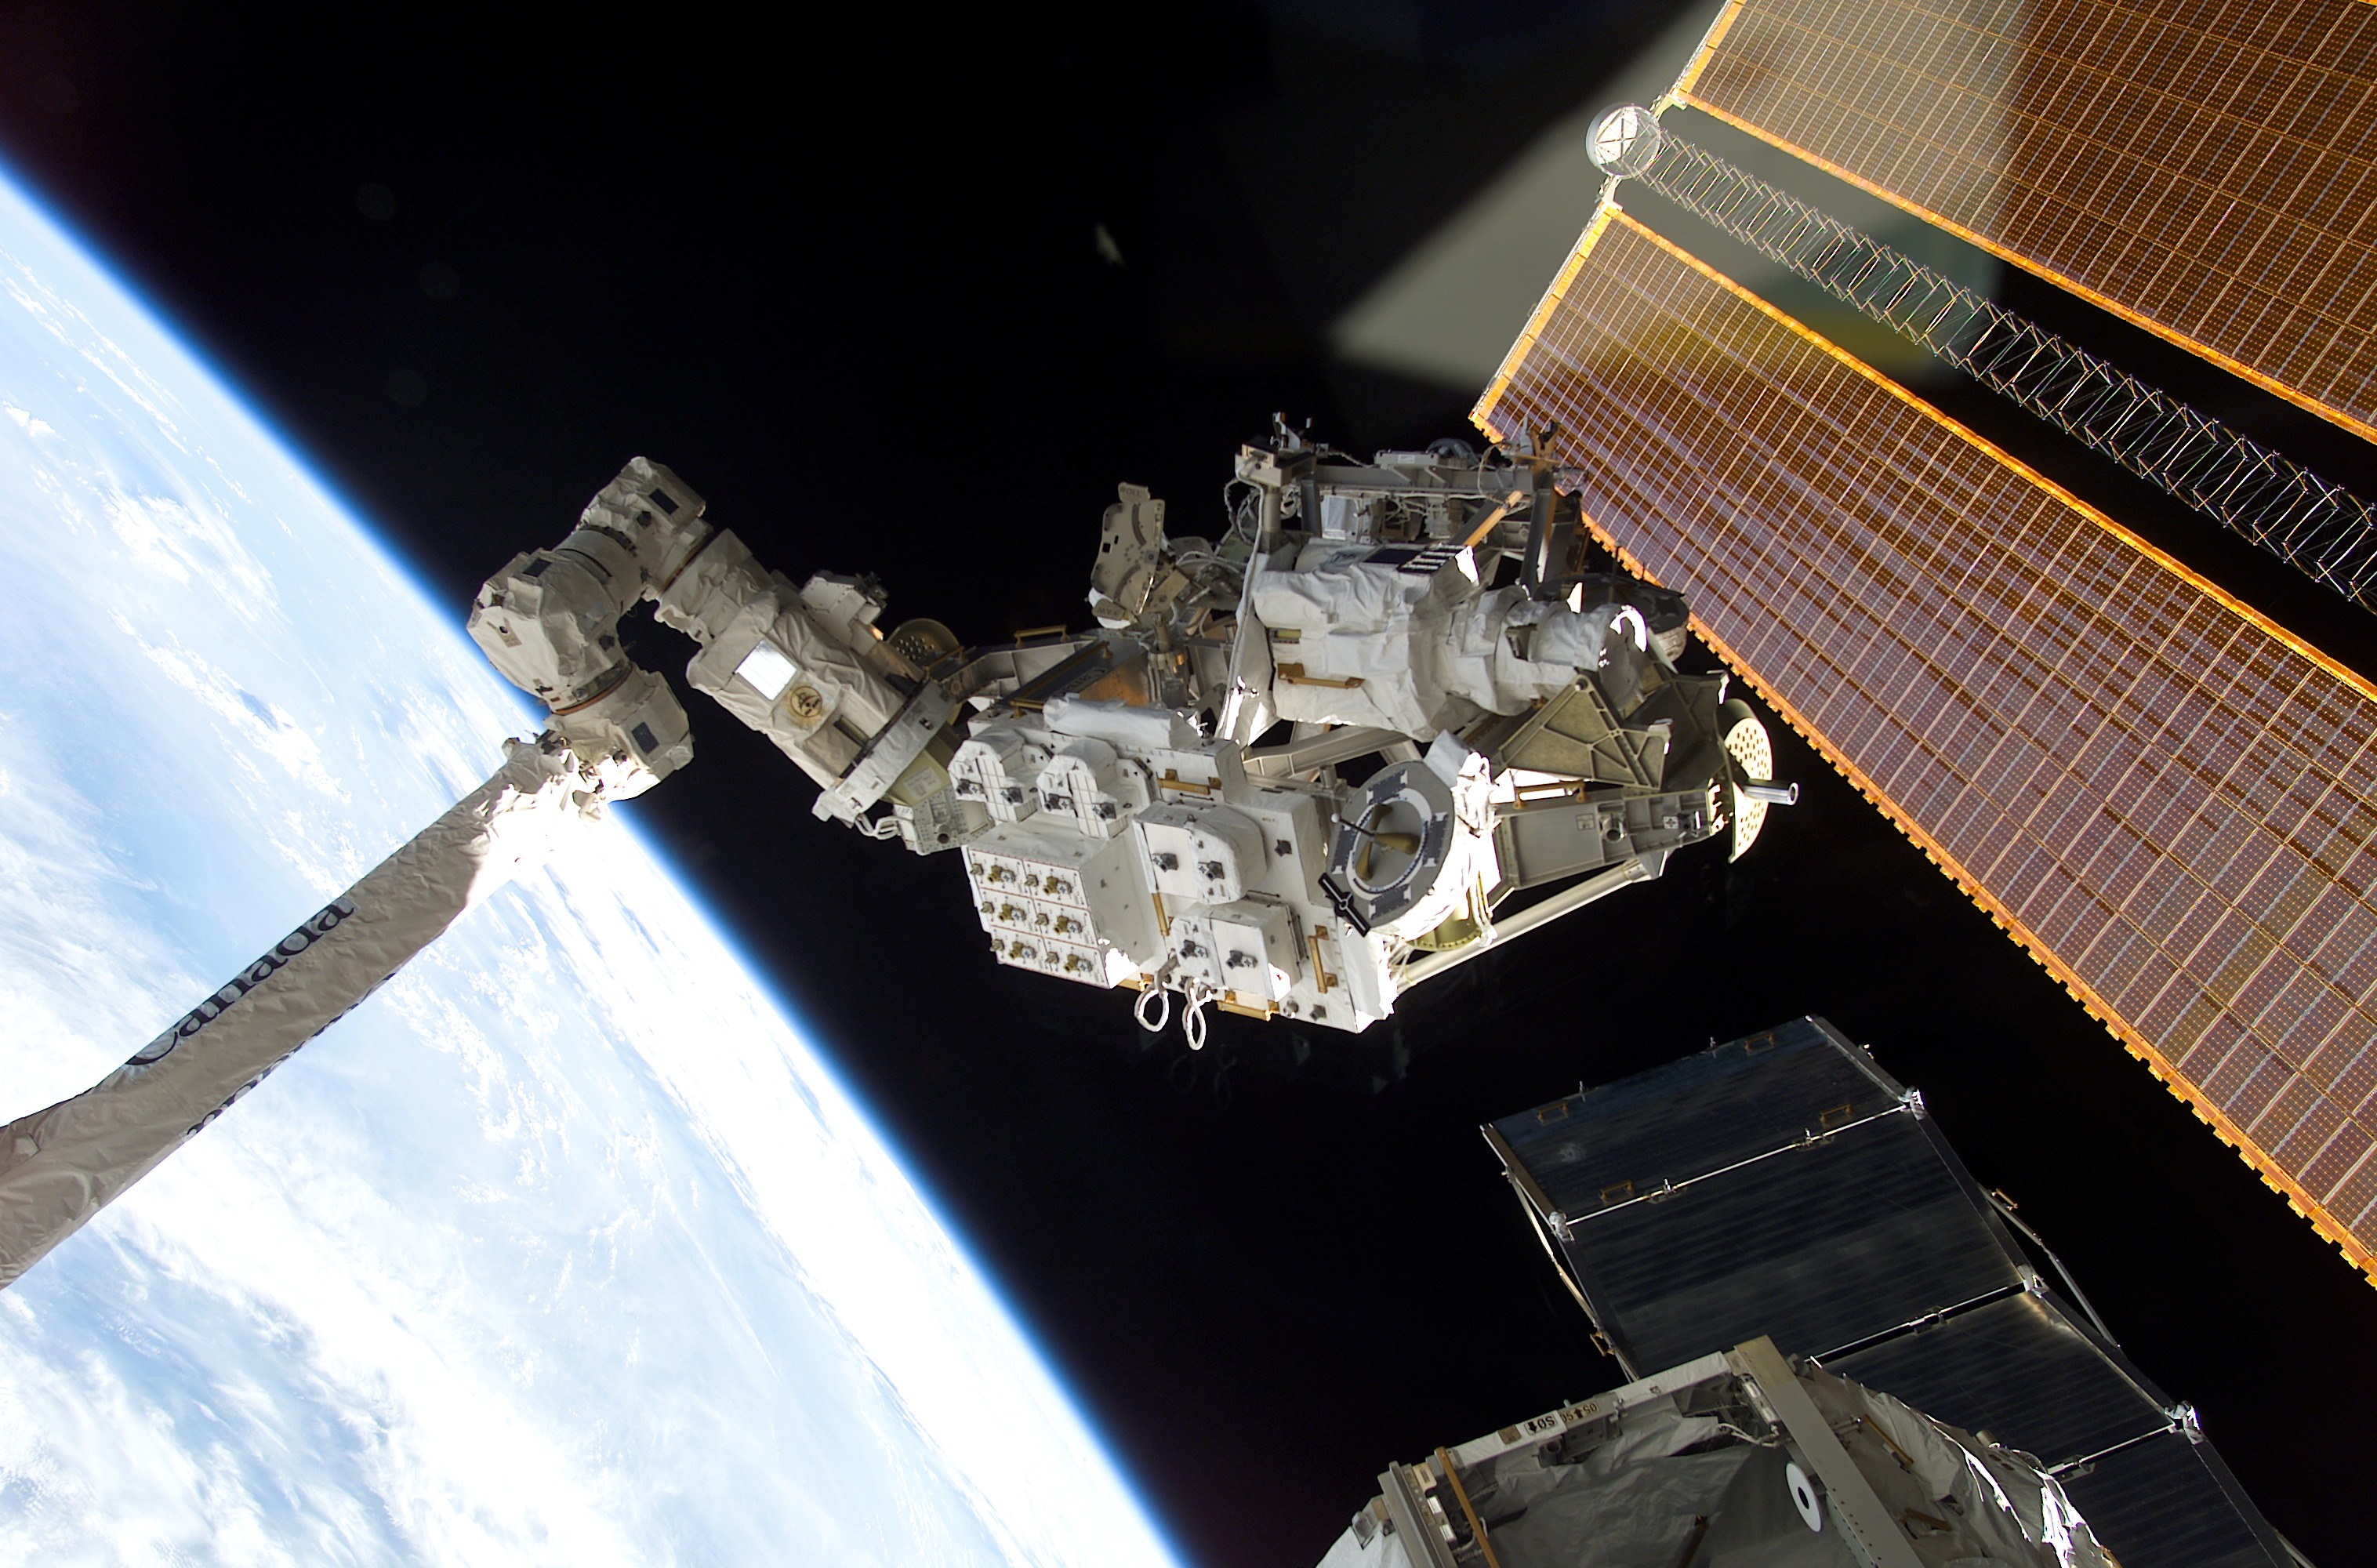
\includegraphics[scale=0.055]{mss}
        \caption{Canadarm2 attached to the Mobile Base System~\cite{mss_wiki}.}
    \end{figure}
\end{column}
\end{columns}
\end{frame}

\begin{frame}{Main Characteristics}
    \begin{columns}
        \begin{column}{0.5 \textwidth}
    \begin{itemize}
        \item Lack of fixed base:
            \begin{itemize}
            \item Free-flying system;
            \item Free-floating system.
            \end{itemize}
        \item Typical capture sequance:
            \begin{enumerate}
                \item observation and planning phase;
                \item final approach phase;
                \item impact and grasping/capture phase;
                \item post-capture stabilization phase.
            \end{enumerate}
        \item To avoid impact: zero relative velocity.
    \end{itemize}
        \end{column} 
        \begin{column}{0.5 \textwidth}
            \begin{figure}
                \centering
                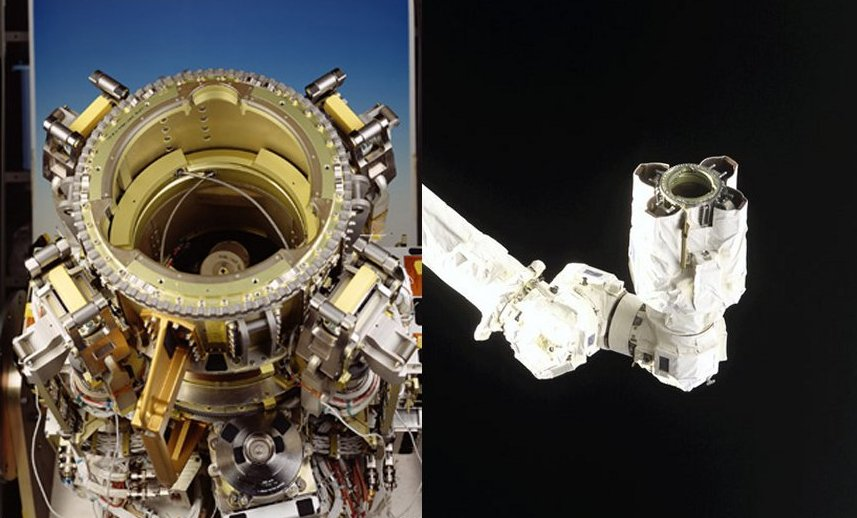
\includegraphics[scale=0.2]{EE.jpg}
                \caption{Latching End Effector (LEE)~\cite{mss_wiki}.}
            \end{figure}
        \end{column}       
    \end{columns}
\end{frame}

\begin{frame}{Main Characteristics}
\begin{columns}
    \begin{column}{0.5\textwidth}
    \begin{itemize}
        \item Two 2-links arms attached to a "shoulder".
        \item Usually redundant kinematics.
        \item Number of degrees of freedom: $n=3(m-1)-2c_1-c_2$
    \end{itemize}
    
    \end{column}
    \begin{column}{0.5\textwidth}
        \begin{figure}
            \centering
            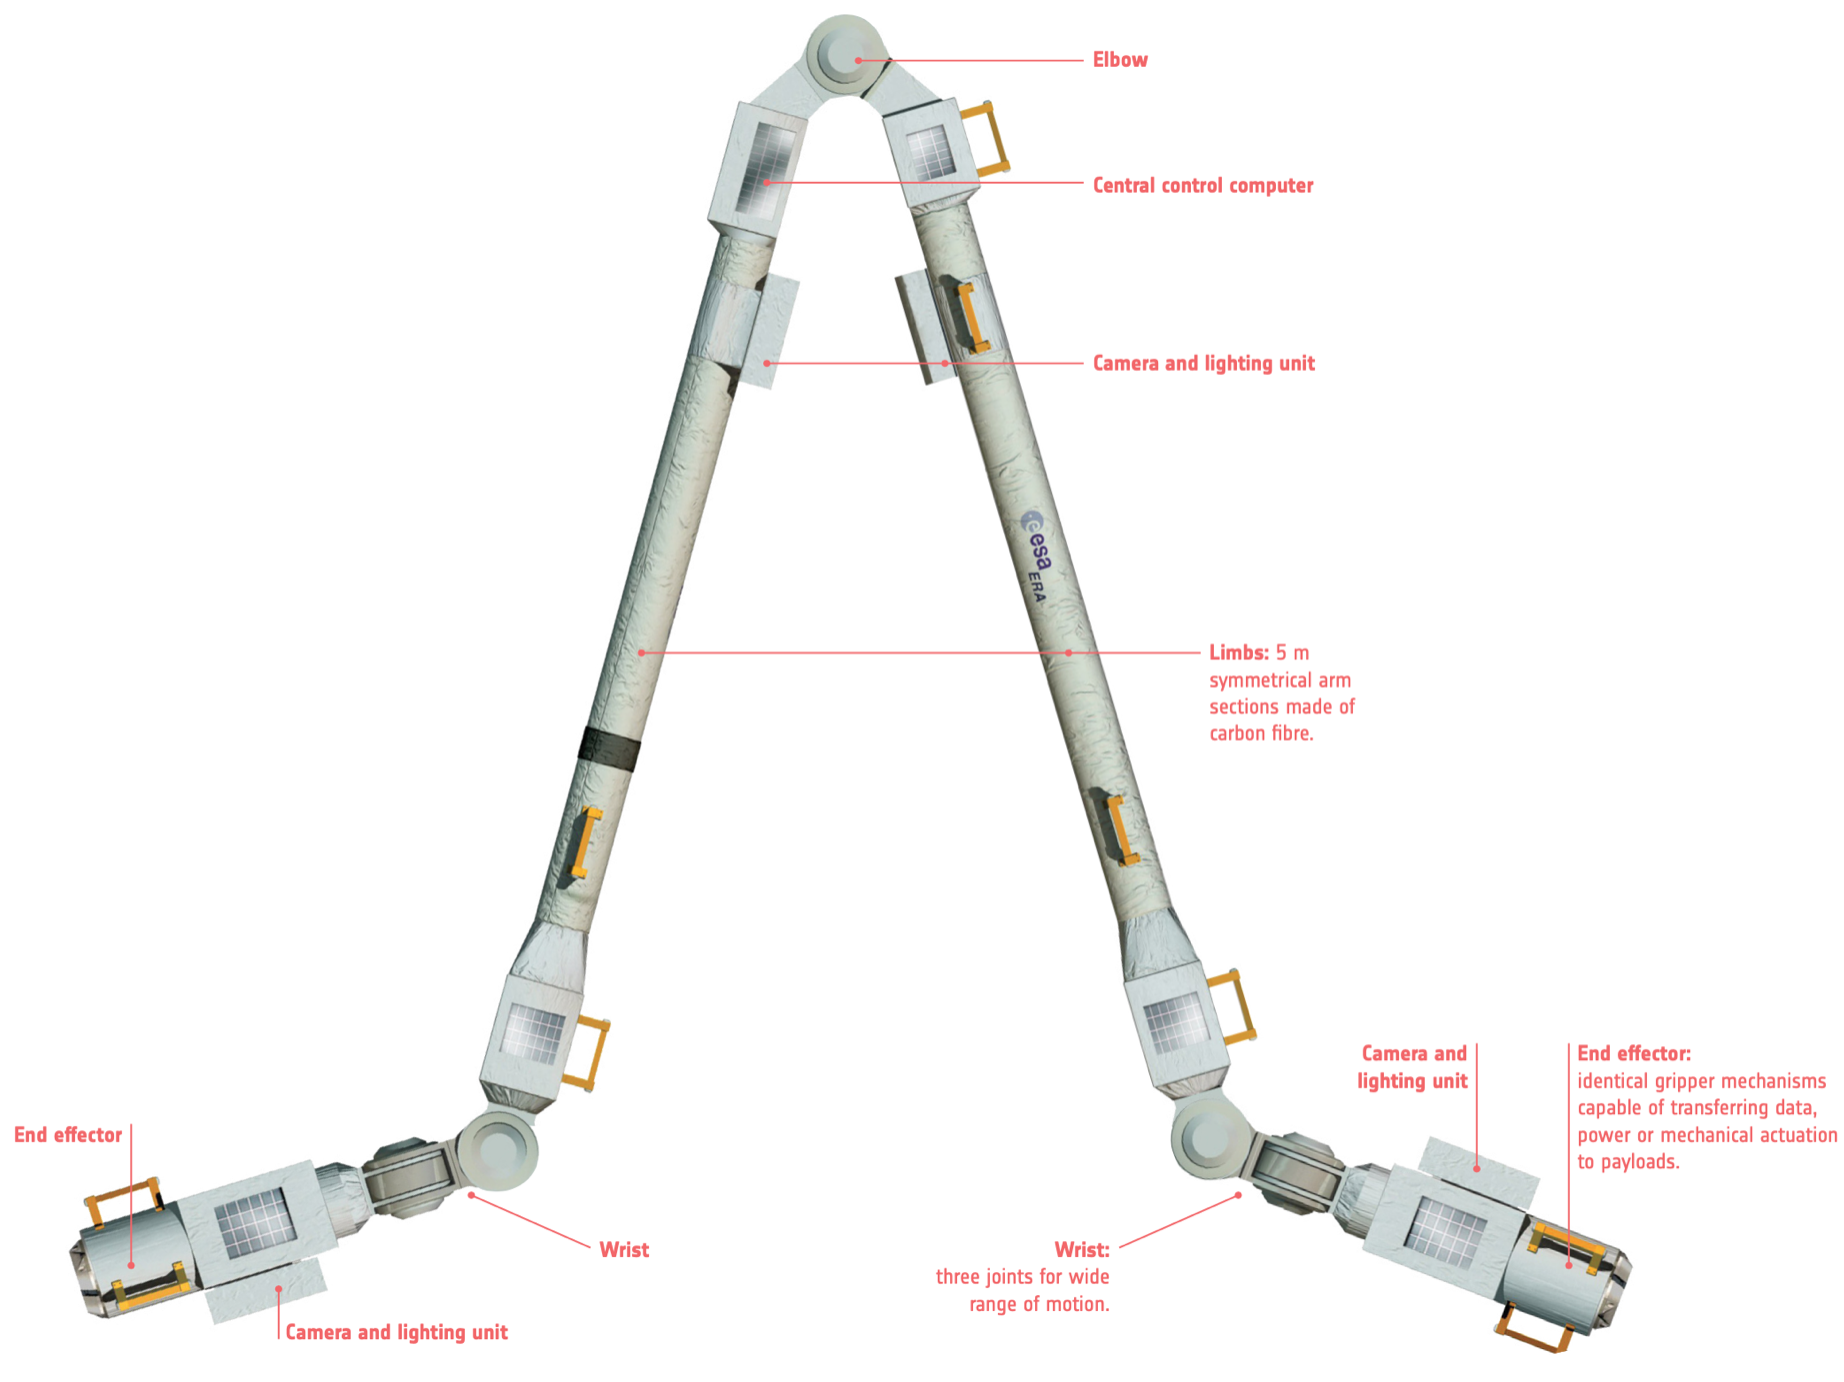
\includegraphics[scale=0.2]{ERA.png}
            \caption{ERA specifications~\cite{era}.}
        \end{figure}
    \end{column}
\end{columns}
\end{frame}

\begin{frame}{State of Art}
    \begin{table}
    \centering
        \begin{tabular}{lccc}
            \hline
        & \textbf{SSRMS} & \textbf{ERA} & \textbf{JEMRMS (MA)}\\
        \hline
        Span&\SI{14.22}{\metre}&\SI{11.3}{\metre}&\SI{9.91}{\metre}\\
        Boom Span&\SI{7.11}{\metre}&\SI{7.77}{\metre}&\SI{3.93}{\metre}\\
        DOFs&7&7&6\\
        Joints&Offset&Inline&Offset\\
        Base&Relocatable&Relocatable&Fixed\\
        Positioning Accuracy&\SI{65}{\milli\metre}, \SI{0.71}{\degree}&\SI{40}{\milli\metre}, \SI{1}{\degree}&\SI{50}{\milli\metre}, \SI{1.8}{\degree}\\
        Mass&\SI{1336}{\kilogram}&\SI{630}{\kilogram}&\SI{757}{\kilogram}\\
        Max Handling Capacity&\SI{116}{\mega\gram}&\SI{8}{\mega\gram}&\SI{7}{\mega\gram}\\
        Power Consumption&\SI{1360}{\watt} (average)&>\SI{800}{\watt}&\SI{2.3}{\kilo\watt}\\
        \hline
        \end{tabular}
    \caption{SSRMS, ERA and JEMRMS specifications~\cite{comparison}.}
    \end{table}
\end{frame}
\section{Kinematics}

\begin{frame}{Fundamentals}
\begin{columns}
    \begin{column}{0.5\textwidth}
        \begin{itemize}
            \item Direct Kinematics.
            \item Inverse Kinematics.
            \item Homogeneous Matrix Approach~\cite{hma1}.
        \end{itemize}
    \end{column}
    \begin{column}{0.5\textwidth}
        \begin{figure}
            \centering
            \scalebox{0.6}{\begin{tikzpicture}

  % Definizione delle lunghezze dei bracci
  \def\lone{4} % Lunghezza del primo braccio
  \def\ltwo{3.5} % Lunghezza del secondo braccio

  % Angoli dei giunti
  \def\thetaone{30} % Angolo del primo giunto (in gradi)
  \def\thetatwo{45} % Angolo del secondo giunto (in gradi)

  % Coordinate del primo giunto
  \coordinate (O) at (0,0);

  % Calcolo delle coordinate del secondo giunto
  \coordinate (A) at ({\lone*cos(\thetaone)},{\lone*sin(\thetaone)});

  % Calcolo delle coordinate dell'end effector
  \coordinate (B) at ({\lone*cos(\thetaone) + \ltwo*cos(\thetaone + \thetatwo)}, 
                      {\lone*sin(\thetaone) + \ltwo*sin(\thetaone + \thetatwo)});

  % Disegno del primo braccio
  \draw[thick, black] (O) -- (A);

  % Disegno del secondo braccio
  \draw[thick, black] (A) -- (B);

  % Disegno assi
  \draw[thick,black,->] (0,0) -- (0,6) node[anchor=east]{y};
    \draw[thick,black,->] (0,0) -- (6,0) node[anchor=west]{x};

  % Rappresentazione dei giunti
  \filldraw[fill=black] (O) circle (0.1); % Base del manipolatore
  \filldraw[fill=black] (A) circle (0.1); % Primo giunto
  \filldraw[fill=red] (B) circle (0.1);   % End effector

  % Etichette
  \node[anchor=east] at (O) {$O$};
  \node[anchor=north] at (A) {$A$};
  \node[anchor=west] at (B) {$B$};

\end{tikzpicture}}
            \caption{2D RR (revolute-revolute) manipulator.}
          \end{figure}
    \end{column}
\end{columns}
\end{frame}

\begin{frame}{Fundamentals}
    \begin{columns}
        \begin{column}{0.5\textwidth}
            \begin{itemize}
                \item Roto-Translation Matrix: \begin{equation}
                    \begin{footnotesize}
                    \prescript{f}{}{\begin{bmatrix}
                      O_fP_x\\
                      O_fP_y\\
                      O_fP_z\\
                      1
                    \end{bmatrix}}=\begin{bmatrix}
                      \prescript{f}{m}{R}&\prescript{f}{}{\begin{bmatrix}
                        O_fO_mx\\
                        O_fO_my\\
                        O_fO_mz\\
                      \end{bmatrix}}\\
                      \mathbf{0}&1
                    \end{bmatrix}\prescript{m}{}{\begin{bmatrix}
                        O_mP_x\\
                        O_mP_y\\
                        O_mP_z\\
                        1
                      \end{bmatrix}}=\prescript{f}{m}{M}\prescript{m}{}{\begin{bmatrix}
                        O_mP_x\\
                        O_mP_y\\
                        O_mP_z\\
                        1
                      \end{bmatrix}}
                    \end{footnotesize}
                  \end{equation}
                \item Veolocity Matrix: $\prescript{f}{}{W}=\prescript{f}{m}{\dot{M}}\prescript{m}{f}{M}$\begin{equation}
                    \begin{footnotesize}
                    W=\begin{bmatrix}
                      0&-\omega_z&\omega_y&v_x\\
                      \omega_z&0&-\omega_x&v_y\\
                      -\omega_y&\omega_x&0&v_z\\
                      0&0&0&0
                    \end{bmatrix}
                    \end{footnotesize}
                  \end{equation}
                \item `Logic Matrix': $ L=\frac{W}{|\omega|}$
            \end{itemize}
        \end{column}
        \begin{column}{0.5\textwidth}
            \begin{figure}
                \centering
                \scalebox{0.6}{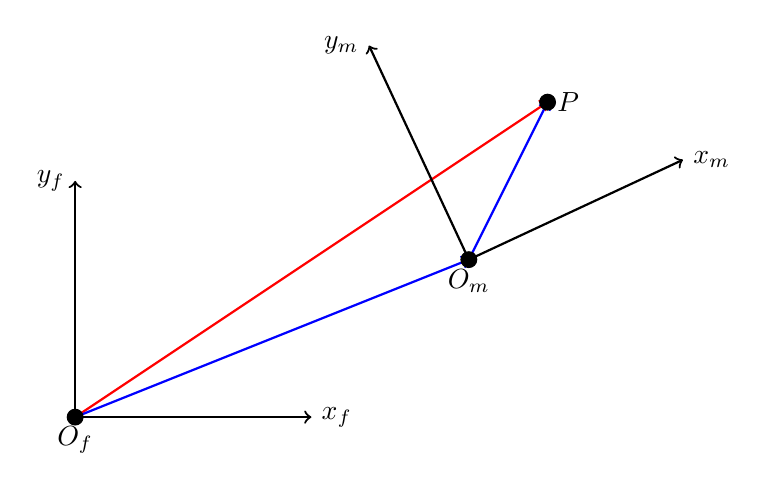
\begin{tikzpicture}

  \def\alpha{25}

  \coordinate (Of) at (0,0);
  \coordinate (Om) at (5,2);
  \coordinate (P) at (6,4);
  \coordinate (xf) at (3,0);
  \coordinate (yf) at (0,3);
  \coordinate (xm) at ({5+3*cos(\alpha)},{2+3*sin(\alpha)});
  \coordinate (ym) at ({5-3*sin(\alpha)},{2+3*cos(\alpha)});

  \draw[thick, red,->,] (Of) -- (P);
  \draw[thick, blue,->] (Of) -- (Om);
  \draw[thick, blue,->] (Om) -- (P);

  \draw[thick,black,->] (Of) -- (yf) node[anchor=east]{$y_f$};
  \draw[thick,black,->] (Of) -- (xf) node[anchor=west]{$x_f$};
  \filldraw[fill=black] (P) circle (0.1);
  \filldraw[fill=black] (Om) circle (0.1);
  \filldraw[fill=black] (Of) circle (0.1);

  \draw[thick,black,->] (Om) -- (ym) node[anchor=east]{$y_m$};
  \draw[thick,black,->] (Om) -- (xm) node[anchor=west]{$x_m$};

  \node[anchor=west] at (P) {$P$};
  \node[anchor=north] at (Om) {$O_m$};
  \node[anchor=north] at (Of) {$O_f$};

\end{tikzpicture}}
                \caption{Definition of a point in a rotated and translated frame with respect to the fixed one.}
              \end{figure}
        \end{column}
    \end{columns}
\end{frame}

\begin{frame}{Danavit-Hartenberg Method}
    \begin{columns}
        \begin{column}{0.5\textwidth}
            \begin{itemize}
                \item Used to define reference frames.
                \item Ordered procedure:
                    \begin{enumerate}
                        \item $z_i$ axis: axis of the revolute joint that connects the link to the following.
                        \item $x_i$ axis: line of minimum distance between $z_{i-1}$ and $z_i$, oriented from $z_{i-1}$ to $z_i$.
                        \item $y_i$ axis: obtained by the vectorial product of the other two axes.
                    \end{enumerate}
            \end{itemize}
        \end{column}
        \begin{column}{0.5\textwidth}
            \begin{figure}
                \centering
                \scalebox{0.4}{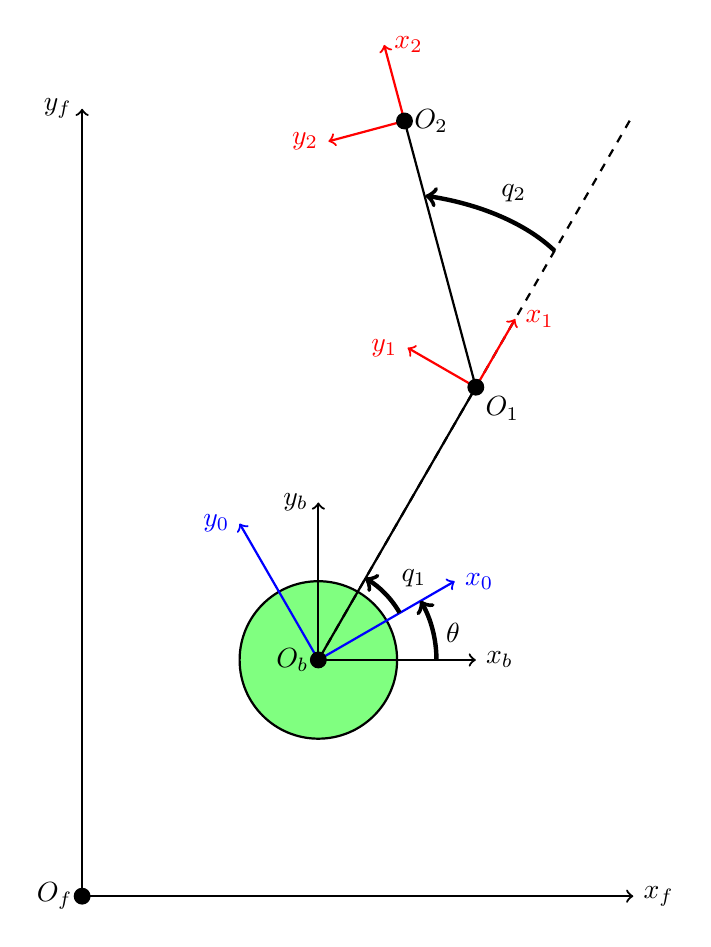
\begin{tikzpicture}

  \def\lone{4} 
  \def\ltwo{3.5}

  \def\thetazero{30}
  \def\thetaone{30}
  \def\thetatwo{45} 

  \coordinate (O) at (0,0);
  \coordinate (Ob) at (3,3);
  \coordinate (Ob0) at ({-0.7+3+2*cos(\thetazero)},{-0.4+3+2*sin(\thetazero)});
  \coordinate (Ob01) at ({-0.8+3+2*cos(\thetazero)},{-0.2+3+2*sin(\thetazero)});
  \coordinate (A) at ({3+\lone*cos(\thetaone+\thetazero)},{3+\lone*sin(\thetaone+\thetazero)});
  \coordinate (C) at ({3+2*\lone*cos(\thetaone+\thetazero)},{3+2*\lone*sin(\thetaone+\thetazero)});
  \coordinate (C0) at ({3+1.5*\lone*cos(\thetaone+\thetazero)},{3+1.5*\lone*sin(\thetaone+\thetazero)});
  \coordinate (C01) at ({3-0.8+1.5*\lone*cos(\thetaone+\thetazero)},{3+0.5+1.5*\lone*sin(\thetaone+\thetazero)});
  \coordinate (B) at ({3+\lone*cos(\thetaone+\thetazero) + \ltwo*cos(\thetaone + \thetatwo+\thetazero)}, 
                      {3+\lone*sin(\thetaone+\thetazero) + \ltwo*sin(\thetaone + \thetatwo+\thetazero)});
  \coordinate (B0) at ({3+1.5*\lone*cos(\thetaone+\thetazero) + 1.5*\ltwo*cos(\thetaone + \thetatwo+\thetazero)}, 
                      {3+1.5*\lone*sin(\thetaone+\thetazero) + 1.5*\ltwo*sin(\thetaone + \thetatwo+\thetazero)});

  \draw[thick,fill=green!50] (3,3) circle (1);

  \draw[thick, black] (Ob) -- (A);
  \draw[thick, black, dashed] (Ob) -- (C);
  \draw[thick, black] (A) -- (B);

  \draw[thick,black,->] (O) -- (0,10) node[anchor=east]{$y_f$};
  \draw[thick,black,->] (O) -- (7,0) node[anchor=west]{$x_f$};

  \draw[thick,black,->] (Ob) -- (3,5) node[anchor=east]{$y_b$};
  \draw[thick,black,->] (Ob) -- (5,3) node[anchor=west]{$x_b$};

  \draw[thick,blue,->] (Ob) -- ({3-2*sin(\thetazero)},{3+2*cos(\thetazero)}) node[anchor=east]{$y_0$};
  \draw[thick,blue,->] (Ob) -- ({3+2*cos(\thetazero)},{3+2*sin(\thetazero)}) node[anchor=west]{$x_0$};
  

  \draw[thick,red,->] (A) -- ({3+\lone*cos(\thetaone+\thetazero)-sin(\thetaone+\thetazero)},{3+\lone*sin(\thetaone+\thetazero)+cos(\thetaone+\thetazero)}) node[anchor=east]{$y_1$};
  \draw[thick,red,->] (A) -- ({3+\lone*cos(\thetaone+\thetazero)+cos(\thetaone+\thetazero)},{3+\lone*sin(\thetaone+\thetazero)+sin(\thetaone+\thetazero)}) node[anchor=west]{$x_1$};

  \draw[thick,red,->] (B) -- ({3+\lone*cos(\thetaone+\thetazero)+ \ltwo*cos(\thetaone + \thetatwo+\thetazero)-sin(\thetaone+ \thetatwo+\thetazero)},{3+\lone*sin(\thetaone+\thetazero)+ \ltwo*sin(\thetaone + \thetatwo+\thetazero)+cos(\thetaone+ \thetatwo+\thetazero)}) node[anchor=east]{$y_2$};
  \draw[thick,red,->] (B) -- ({3+\lone*cos(\thetaone+\thetazero)+ \ltwo*cos(\thetaone + \thetatwo+\thetazero)+cos(\thetaone+ \thetatwo+\thetazero)},{3+\lone*sin(\thetaone+\thetazero)+ \ltwo*sin(\thetaone + \thetatwo+\thetazero)+sin(\thetaone+ \thetatwo+\thetazero)}) node[anchor=west]{$x_2$};

  \draw[ultra thick,->] (4.5,3) arc [start angle=0, end angle=\thetaone, x radius=1.5, y radius=1.5];
  \draw[ultra thick,->] (Ob0) arc [start angle=\thetazero, end angle={\thetaone+\thetazero}, x radius=1.2, y radius=1.2];
  \draw[ultra thick,->] (C0) arc [start angle=\thetaone, end angle={\thetatwo+\thetaone}, x radius=2.7, y radius=1.5];

  \filldraw[fill=black] (O) circle (0.1);
  \filldraw[fill=black] (Ob) circle (0.1);
  \filldraw[fill=black] (A) circle (0.1);
  \filldraw[fill=black] (B) circle (0.1);

  \node[anchor=east] at (O) {$O_f$};
  \node[anchor=east] at (Ob) {$O_b$};
  \node[anchor=north west] at (A) {$O_1$};
  \node[anchor=west] at (B) {$O_2$};
  \node[anchor=south west] at (4.5,3.1) {$\theta$};
  \node[anchor=south west] at (Ob01) {$q_1$};
  \node[anchor=south west] at (C01) {$q_2$};

\end{tikzpicture}}
                \caption{The Danavit-Hartenberg rule has been used to place the local joints' frame (in red) in a planar RR manipulator.}
              \end{figure}
        \end{column}
    \end{columns}
\end{frame}

\begin{frame}{Planar VMS}
    \begin{itemize}
        \item VMS' coordinates: $p=\{x_b,y_b,\theta_b,q_1,q_2\}$
        \item Satellite coordinates: $  \psi=\{x_O,y_O,\theta_O\}$
    \end{itemize}
    \vspace{0.5cm}
        \begin{equation}
            \begin{footnotesize}
            \begin{array}{c}
              \prescript{f}{b}{M}=\begin{bmatrix}
              1&0&0&x_b\\
              0&1&0&y_b\\
              0&0&1&0\\
              0&0&0&1
              \end{bmatrix}\quad
              \prescript{b}{0}{M}=\begin{bmatrix}
                \cos{\theta_0}&-\sin{\theta_0}&0&0\\
                \sin{\theta_0}&\cos{\theta_0}&0&0\\
                0&0&1&0\\
                0&0&0&1
              \end{bmatrix}\\ \\
              \prescript{0}{1}{M}=\begin{bmatrix}
                \cos{q_1}&-\sin{q_1}&0&l_1\cos{q_1}\\
                \sin{q_1}&\cos{q_1}&0&l_1\sin{q_1}\\
                0&0&1&0\\
                0&0&0&1
              \end{bmatrix}\quad
              \prescript{1}{2}{M}=\begin{bmatrix}
                \cos{q_2}&-\sin{q_2}&0&l_2\cos{q_2}\\
                \sin{q_2}&\cos{q_2}&0&l_2\sin{q_2}\\
                0&0&1&0\\
                0&0&0&1
              \end{bmatrix}
            \end{array}
            \end{footnotesize}
          \end{equation}
\end{frame}

\begin{frame}{Planar VMS}
    \begin{equation}
        \begin{footnotesize}
        p_{EE}=\prescript{0}{2}{M}O_3= \begin{bmatrix}
          l_1\cos{(\theta_0+q_1)}+l_2\cos{(\theta_0+q_1+q_2)}+x_b\\
          l_1\sin{(\theta_0+q_1)}+l_2\sin{(\theta_0+q_1+q_2)}+y_b\\0\\1
         \end{bmatrix}
        \end{footnotesize}
      \end{equation}
with $O_3=\{0,0,0,1\}$.
\begin{equation}
    \begin{footnotesize}
    \begin{array}{c}
      \prescript{f}{}{W_{{f1}_{1:3,1:3}}}=\begin{bmatrix}
        0&-\theta_0-q_1&0\\
        \theta_0+q_1&0&0\\
        0&0&0
      \end{bmatrix} \quad
      \prescript{f}{}{W_{{f2}_{1:3,1:3}}}=\begin{bmatrix}
        0&-\theta_0-q_1-q_2&0\\
        \theta_0+q_1+q_2&0&0\\
        0&0&0
      \end{bmatrix}
    \end{array}
    \end{footnotesize}
  \end{equation}
  \begin{equation}
  \begin{footnotesize}
    \begin{array}{c}
      \prescript{f}{}{L_{{f1}_{1:3,1:3}}}=\begin{bmatrix}
        0&-1&0\\
        1&0&0\\
        0&0&0
      \end{bmatrix} \quad
      \prescript{f}{}{L_{{f2}_{1:3,1:3}}}=\begin{bmatrix}
        0&-1&0\\
        1&0&0\\
        0&0&0
      \end{bmatrix}
    \end{array}
    \end{footnotesize}
  \end{equation}
\end{frame}

\begin{frame}{Satellite Kinematics}
    \begin{columns}
        \begin{column}{0.5\textwidth}
            \begin{equation}
                \begin{footnotesize}
                \begin{array}{c}
                  \prescript{f}{O_0}{M}=\begin{bmatrix}
                    1&0&0&x_O\\
                  0&1&0&y_O\\
                  0&0&1&0\\
                  0&0&0&1
                  \end{bmatrix}\quad
                  \prescript{O_0}{O_1}{M}=\begin{bmatrix}
                    \cos{\theta_O}&-\sin{\theta_O}&0&0\\
                    \sin{\theta_O}&\cos{\theta_O}&0&0\\
                    0&0&1&0\\
                    0&0&0&1
                  \end{bmatrix}\\
                  \\
                  \prescript{O_1}{O_2}{M}=\begin{bmatrix}
                    \cos{\gamma}&-\sin{\gamma}&0&r \cos{\gamma}\\
                    \sin{\gamma}&\cos{\gamma}&0&r \sin{\gamma}\\
                    0&0&1&0\\
                    0&0&0&1
                  \end{bmatrix}
                \end{array}            
            \end{footnotesize}
              \end{equation}
        \end{column}
        \begin{column}{0.5\textwidth}
            \begin{figure}
                \centering
                \scalebox{0.6}{\begin{tikzpicture}

  \def\thetaO{30}
  \def\alpha{60}
  \def\r{2}

  \coordinate (O) at (0,0);
  \coordinate (Oo) at (3,3);
  \coordinate (cp) at ({3+\r*cos(\alpha)},{3+\r*sin(\alpha)});

  \draw[thick,fill=red!50] (3,3) circle (\r);

  \draw[thick,black,->] (O) -- (0,7) node[anchor=east]{$y_f$};
  \draw[thick,black,->] (O) -- (7,0) node[anchor=west]{$x_f$};

  \draw[thick,black,->] (Oo) -- (3,6) node[anchor=east]{$y_{O_0}$};
  \draw[thick,black,->] (Oo) -- (6,3) node[anchor=west]{$x_{O_0}$};

  \draw[thick,black,->] (Oo) -- ({3-3*sin(\thetaO)},{3+3*cos(\thetaO)}) node[anchor=east]{$y_{O_1}$};
  \draw[thick,black,->] (Oo) -- ({3+3*cos(\thetaO)},{3+3*sin(\thetaO)}) node[anchor=west]{$x_{O_1}$};

  \draw[thick,white] (Oo) -- ({3+\r*cos(\alpha)},{3+\r*sin(\alpha)}) node[anchor=north east]{$r$};

  \draw[ultra thick,->] (5.5,3) arc [start angle=0, end angle=\thetaO, x radius=2.5, y radius=2.5];
  \draw[ultra thick,->] ({3+1.3*cos(\thetaO)},{3+1.3*sin(\thetaO)}) arc [start angle=0, end angle=\alpha, x radius=0.7, y radius=0.7];

  \filldraw[fill=black] (O) circle (0.1);
  \filldraw[fill=black] (Oo) circle (0.1);
  \filldraw[fill=black] (cp) circle (0.1);

  \node[anchor=east] at (O) {$O_f$};
  \node[anchor=east] at (Ob) {$O_{O_0}$};
  \node[anchor=south west] at (5.5,3.3) {$\theta_O$};
  \node[anchor=east] at ({3+1.8*cos(\thetaO)},{3+2.2*sin(\thetaO)}) {$\gamma$};
  \node[anchor=south west] at (cp) {$c_p$};

\end{tikzpicture}}
                \caption{Tumbling object disk approximation.}
              \end{figure}
        \end{column}
    \end{columns}
\end{frame}

\section{Dynamics}

\begin{frame}{Fundamentals}
    \begin{itemize}
        \item Direct Dynamics.
        \item Inverse Dynamics.
        \item Given a \textit{wrench} \textbf{w} at the EE:
        \begin{itemize}
            \item Power at the joints: $P_{\tau}=\tau_w^T\dot{q}$
            \item Power at the EE: $P_e=w^Tv$
            \item Conservation of energy: \\
            \vspace{2mm}
            $P_{\tau}=P_e \quad \Rightarrow \quad  \tau_w^T\dot{q}=w^Tv=w^TJ\dot{q} \quad \forall\dot{q}\Rightarrow \quad  \tau_w^T=w^TJ \quad \Rightarrow \quad \tau_w=J^Tw $
        \end{itemize}
        \vspace{1mm}
        \item Equation of motion: $ M(q)\ddot{q}+C(q,\dot{q})=u+J^T(q)w$
    \end{itemize}
\end{frame}

\begin{frame}{VMS}
\begin{itemize}
    \item Homogeneous Matrix Approach~\cite{hma1,hma2}.
    \item Lagrangian formulation: 
    \begin{equation} 
        \mathcal{L} (q,\dot{q}) = \sum_{i=1}^NT_i-U_i, \quad  \frac{d}{dt}\frac{\partial \mathcal{L} }{\partial \dot{q}_i}-\frac{\partial \mathcal{L} }{\partial q_i}=f_i 
    \end{equation}
    \item Pseudo Inertia Tensor: 
    \begin{equation}
        \begin{footnotesize}
        \prescript{i}{}{J_k}=\begin{bmatrix}
            J_{xx}&J_{xy}&J_{xz}&m_kx_G\\
            J_{yx}&J_{yy}&J_{yz}&m_ky_G\\
            J_{zx}&J_{zy}&J_{zz}&m_kz_G\\
            m_kx_G&m_ky_G&m_kz_G&m
        \end{bmatrix}                 
        \end{footnotesize}
    \end{equation}
    with \begin{equation}
        \begin{footnotesize}
        \begin{array}{c}
            J_{xx}=\int x^2\,dm\quad J_{yy}=\int y^2\,dm\quad J_{zz}=\int z^2\,dm\\
            J_{xy}=\int xy\,dm\quad J_{xz}=\int xz\,dm\quad J_{yz}=\int yz\,dm
        \end{array}
        \end{footnotesize}
        \end{equation}
\end{itemize}
\end{frame}

\begin{frame}{VMS}
    \begin{columns}
        \begin{column}{0.5\textwidth}
            \begin{itemize}
                \item Action Matrix:
                \begin{equation}
                    \begin{footnotesize}
                    \prescript{i}{}{\phi}_k=\begin{bmatrix}
                      0&-c_z&c_y&f_x\\
                      c_z&0&-c_x&f_y\\
                      -c_y&c_x&0&f_z\\
                      -f_x&-f_y&-f_z&0
                    \end{bmatrix}
                    \end{footnotesize}
                  \end{equation}
                \item Non-Lagrangian components:
                \begin{equation}
                    f_{q_i}=\Big(\sum_{j=1}^N\prescript{f}{}{\phi_j}\Big)\otimes \prescript{f}{}{L_{q_i}}
                  \end{equation}
            \end{itemize}
        \end{column}
        \begin{column}{0.5\textwidth}
            \begin{figure}
                \centering
                \scalebox{0.55}{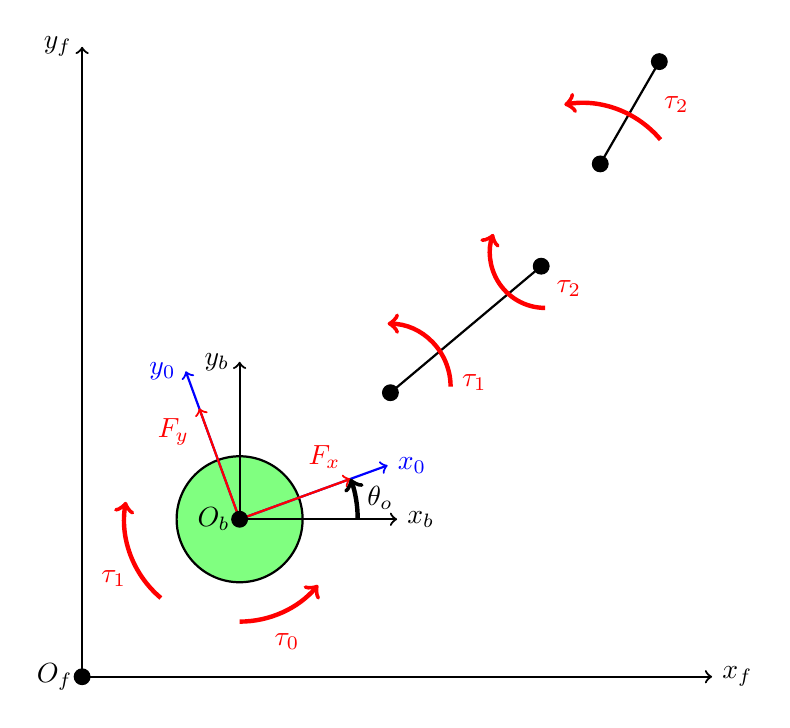
\begin{tikzpicture}

  \def\lone{5} 
  \def\ltwo{3}

  \def\thetazero{20}
  \def\thetaone{20}
  \def\thetatwo{20} 

  \coordinate (O) at (0,0);
  \coordinate (Ob) at (2,2);
  \coordinate (q) at (1,1);
  \coordinate (A') at ({2+\lone/2*cos(\thetaone+\thetazero)},{2+\lone/2*sin(\thetaone+\thetazero)});
  \coordinate (Ob0) at ({-0.2+3+2*cos(\thetazero)},{3+2*sin(\thetazero)});
  \coordinate (Ob00) at ({4+2*cos(\thetazero)},{4+2*sin(\thetazero)});
  \coordinate (Ob01) at ({-0.2+3+2*cos(\thetazero)},{-0.2+3+2*sin(\thetazero)});
  \coordinate (Ob02) at ({4+2*cos(\thetazero)},{4+2*sin(\thetazero)});
  \coordinate (A) at ({2+\lone*cos(\thetaone+\thetazero)},{2+\lone*sin(\thetaone+\thetazero)});
  \coordinate (C) at ({2+2*\lone*cos(\thetaone+\thetazero)},{2+2*\lone*sin(\thetaone+\thetazero)});
  \coordinate (C0) at ({1.6+1.5*\lone*cos(\thetaone+\thetazero)},{2+1.5*\lone*sin(\thetaone+\thetazero)});
  \coordinate (C01) at ({1.5+1.5*\lone*cos(\thetaone+\thetazero)},{2.2+1.5*\lone*sin(\thetaone+\thetazero)});
  \coordinate (B') at ({2+\lone*cos(\thetaone+\thetazero) + \ltwo/2*cos(\thetaone + \thetatwo+\thetazero)}, 
                      {2+\lone*sin(\thetaone+\thetazero) + \ltwo/2*sin(\thetaone + \thetatwo+\thetazero)});
  \coordinate (B) at ({2+\lone*cos(\thetaone+\thetazero) + \ltwo*cos(\thetaone + \thetatwo+\thetazero)}, 
                      {2+\lone*sin(\thetaone+\thetazero) + \ltwo*sin(\thetaone + \thetatwo+\thetazero)});
  \coordinate (B0) at ({3+1.5*\lone*cos(\thetaone+\thetazero) + 1.5*\ltwo*cos(\thetaone + \thetatwo+\thetazero)}, 
                      {3+1.5*\lone*sin(\thetaone+\thetazero) + 1.5*\ltwo*sin(\thetaone + \thetatwo+\thetazero)});

  \draw[thick,fill=green!50] (2,2) circle (0.8);

  \draw[thick, black] (A') -- (A);
  \draw[thick, black] (B') -- (B);

  \draw[thick,black,->] (O) -- (0,8) node[anchor=east]{$y_f$};
  \draw[thick,black,->] (O) -- (8,0) node[anchor=west]{$x_f$};

  \draw[thick,black,->] (Ob) -- (2,4) node[anchor=east]{$y_b$};
  \draw[thick,black,->] (Ob) -- (4,2) node[anchor=west]{$x_b$};

  \draw[thick,blue,->] (Ob) -- ({2-2*sin(\thetazero)},{2+2*cos(\thetazero)}) node[anchor=east]{$y_0$};
  \draw[thick,blue,->] (Ob) -- ({2+2*cos(\thetazero)},{2+2*sin(\thetazero)}) node[anchor=west]{$x_0$};

  \draw[thick,red,->] (Ob) -- ({2-1.5*sin(\thetazero)},{2+1.5*cos(\thetazero)}) node[anchor=north east]{$F_y$};
  \draw[thick,red,->] (Ob) -- ({2+1.5*cos(\thetazero)},{2+1.5*sin(\thetazero)}) node[anchor=south east]{$F_x$};
  

  \draw[ultra thick,->,red] (2,0.7) arc [start angle=-90, end angle=-40, x radius=1.3, y radius=1.3] node[anchor=south west] at (2.3,0.2) {$\tau_0$};
  \draw[ultra thick,->,red] (q) arc [start angle=-130, end angle=-190, x radius=1.3, y radius=1.3] node[anchor=south west] at (0.1,1) {$\tau_1$};
  \draw[ultra thick,->] (3.5,2) arc [start angle=0, end angle=\thetaone, x radius=1.5, y radius=1.5];
  \draw[ultra thick,->,red] (Ob0) arc [start angle=0, end angle={\thetaone+\thetazero+50}, x radius=0.8, y radius=0.8] node[anchor=south west] at (Ob01) {$\tau_1$};
  \draw[ultra thick,->,red] (Ob00) arc [start angle=-90, end angle=-200, x radius=0.7, y radius=0.7] node[anchor=south west] at (Ob02) {$\tau_2$};
  \draw[ultra thick,->, red] (C0) arc [start angle=\thetaone+20, end angle={\thetatwo+\thetaone+60}, x radius=1.3, y radius=1.3] node[anchor=south west] at (C01) {$\tau_2$};

  \filldraw[fill=black] (O) circle (0.1);
  \filldraw[fill=black] (Ob) circle (0.1);
  \filldraw[fill=black] (A') circle (0.1);
  \filldraw[fill=black] (A) circle (0.1);
  \filldraw[fill=black] (B) circle (0.1);
  \filldraw[fill=black] (B') circle (0.1);

  \node[anchor=east] at (O) {$O_f$};
  \node[anchor=east] at (Ob) {$O_b$};
  \node[anchor=south west] at (3.5,2) {$\theta_o$};

\end{tikzpicture}}
                \caption{Forces and torques applied to the base and to the links.}
              \end{figure}
        \end{column}
    \end{columns}
    \end{frame}

    \begin{frame}{VMS}
        \begin{columns}
            \begin{column}{0.5\textwidth}
                \begin{itemize}
                    \item Non-Lagrangian components:
                    \begin{equation}
                        \begin{footnotesize}
                        \begin{array}{l}
                        f_1=\Big(\prescript{f}{}{\phi_b}+\prescript{f}{}{\phi_1}+\prescript{f}{}{\phi_2}\Big)\otimes \prescript{f}{}{L_{fb_x}}=F_x\cos{\theta_0}-F_y\sin{\theta_0}\\
                        f_2=\Big(\prescript{f}{}{\phi_b}+\prescript{f}{}{\phi_1}+\prescript{f}{}{\phi_2}\Big)\otimes \prescript{f}{}{L_{fb_y}}=F_x\sin{\theta_0}+F_y\cos{\theta_0}\\
                        f_3=\Big(\prescript{f}{}{\phi_b}+\prescript{f}{}{\phi_1}+\prescript{f}{}{\phi_2}\Big)\otimes \prescript{f}{}{L_{f0}}=\tau_0\\
                        f_4=\Big(\prescript{f}{}{\phi_b}+\prescript{f}{}{\phi_1}\Big)\otimes \prescript{f}{}{L_{01}}=\tau_1\\
                        f_5=\prescript{f}{}{\phi_b}\otimes \prescript{f}{}{L_{12}}=\tau_2
                        \end{array}
                    \end{footnotesize}
                      \end{equation}
                    \item Kinetic Energy
                    \begin{equation}
                          T_j=\frac{1}{2}\Tr{\Big(\prescript{f}{}{W_{fj}}\prescript{f}{}{J_j}\prescript{f}{}{W_{fj}^T}\Big)}
                      \end{equation} 
                \end{itemize}
            \end{column}
            \begin{column}{0.5\textwidth}
                \begin{table}
                    \caption{Moments of inertia of the planar VMS' bodies, with respect to their centre of mass (in the centre of the base and the arms), with $i=\{1,2\}$.}
                    \begin{center}
                    \begin{tabular}{lccc}
                    \hline
                    \textbf{Body} & \textbf{Tensor of Pseudo Inertia}\\
                    \hline
                    Base&$\begin{bmatrix}
                      \frac{1}{4}m_br^2&0&0\\
                      0&\frac{1}{4}m_br^2&0\\
                      0&0&0
                    \end{bmatrix}$\\
                    \\
                    Arms&$\begin{bmatrix}
                      \frac{1}{3}m_il_i^2&0&0\\
                      0&0&0\\
                      0&0&0
                    \end{bmatrix}$\\
                    \hline
                    \end{tabular}
                    \end{center}
                    \end{table}
            \end{column}
        \end{columns}
        \end{frame}

\begin{frame}{Satellite}
    \begin{itemize}
        \item Same procedure or, alternatively:
        \begin{equation}
            T_O=v_Om_Ov_O^T+\frac{1}{2}I_{O_z}\theta_O^2
          \end{equation}
        \item Mass matrix: 
        \begin{equation}
            M_O=\begin{bmatrix}
                m_O&0&0\\
                0&m_O&0\\
                0&0&\frac{m_Or^2}{2}
              \end{bmatrix}
        \end{equation}
    \end{itemize}
\end{frame}

\section{Impact Analysis}

\begin{frame}{Conservation of Momentum}
    \begin{itemize}
        \item Four assumptions~\cite{1997}: \begin{itemize}
            \item Only the generalized velocities change during the impat, no displacement.
            \item At the contact point between the end-effector and the target there are no forces but moments only.
            \item We know the satellite's mass and initial velocities.
            \item Plastic impact.
        \end{itemize}
        \item Equations of motion: \begin{equation}
                \begin{cases}
                  M\ddot{p}+C=u+J^Tf_I\\
                  M_O\ddot{\psi}+C_O=-J_O^Tf_I
                \end{cases}
              \end{equation}
              and \begin{equation}
                \int_{0}^{\pi}M\ddot{p}\,dt+\int_{0}^{\pi}C\,dt =-\int_{0}^{\pi}J^T(J_O^+)^TM_O\ddot{\psi}_O\,dt+\int_{0}^{\pi}(u-J^T(J_O^+)^TC_O)\,dt
              \end{equation}
    \end{itemize}
\end{frame}

\begin{frame}{Conservation of Momentum}
\begin{itemize}
    \item Conservation of momentum equation:
    \begin{equation}
        M(\dot{p}_f-\dot{p}_i)+J^T(J_O^+)^TM_O(\dot{\psi}_f-\dot{\psi_i})=0
        \label{conservation}
      \end{equation}
    \item For one degree of freedom:
    \begin{equation}
        m_1(v_{f,1}-v_{i,1})+m_2(v_{f,2}-v_{i,2})=0
      \end{equation}
\end{itemize}    
\end{frame}

\begin{frame}{Rigid Bodies}
    \begin{itemize}
        \item For plastic impacts:
        \begin{equation}
            J\dot{p_f}=J_O\dot{\psi_f} \quad \Rightarrow \quad  \dot{\psi}_f=J_O^+J\dot{p}_f
            \label{contact}
          \end{equation}
        \item Substituting (\ref{contact}) in (\ref{conservation}):
        \begin{equation}
            \dot{p}_f=G^{-1}H
        \end{equation}
        where:
        \begin{equation}
            \begin{array}{l}
              G=M+J^T(J_O^+)^TM_OJ_O^+J\\
              H=M\dot{p}_i+J^T(J_O^+)^TM_O\dot{\psi}_i
            \end{array}
          \end{equation}
    \end{itemize}
\end{frame}

\begin{frame}{Rigid Bodies}
    \begin{itemize}
        \item New equation after impact:
        \begin{equation}
            \dot{\psi}_f=J_O^+J\dot{p}_f \quad \Rightarrow \quad \ddot{\psi}=J_O^+J\ddot{p}+\frac{\partial J_O^+}{\partial t}J\dot{p}+J_O^+\frac{\partial J}{\partial t}\dot{p}
        \end{equation}
        \begin{equation*}
            \begin{cases}
              M\ddot{p}+C=u+J^Tf_I\\
              M_O\ddot{\psi}+C_O=-J_O^Tf_I
            \end{cases}
          \end{equation*}
          \begin{equation}
            M'\ddot{p}+C'=u
          \end{equation}
          where:
        \begin{equation}
        \begin{array}{l}
            M'=M+J^T(J_O^T)^+M_OJ_O^+J\\
            C'=C+J^T(J_O^T)^+M_O\frac{\partial J_O^+}{\partial t}J\dot{p}+J^T(J_O^T)^+M_OJ^+\frac{\partial J}{\partial t}\dot{p}+J^T(J_O^T)^+C_O
        \end{array}
        \end{equation}
    \end{itemize}
\end{frame}

\begin{frame}{Rigid Bodies}
    \begin{table}
        \caption{VMS parameters.}
        \begin{center}
        \begin{tabular}{cccccccc}
            \hline
            $l_1$&$l_2$&$m_b$&$m_1$&$m_2$&$m_O$&$r$&$\gamma$\\
        \hline
            \SI{5.59}{\metre}&\SI{5.59}{\metre}&\SI{419725}{\kilogram}&\SI{300}{\kilogram}&\SI{300}{\kilogram}&\SI{3000}{\kilogram}&\SI{0.12}{\metre}&\SI{0.5}{\radian}\\
        \hline
        \end{tabular}
        \end{center}
        \end{table}
        \begin{table}
        \caption{Simulation's initial positions.}
        \begin{center}
        \begin{tabular}{cccccccc}
            \hline
            $x_b$&$y_b$&$\theta_0$&$q_1$&$q_2$&$x_O$&$y_O$&$\theta_O$\\
        \hline
            \SI{4}{\metre}&\SI{2}{\metre}&\SI[parse-numbers = false]{\pi/2}{\radian}&\SI{0}{\radian}&\SI[parse-numbers = false]{\pi/2}{\radian}&\SI{-1.71}{\metre}&\SI{7.59}{\metre}&\SI{5.78}{\radian}\\
        \hline
        \end{tabular}
        \end{center}
        \end{table}
\end{frame}

\begin{frame}{Rigid Bodies}
    \begin{columns}
        \begin{column}{0.5\textwidth}
            \begin{table}
                \caption{Simulation's initial velocities.}
                \begin{center}
                \begin{tabular}{lcc}
                    \hline
                    &\textbf{Simulation 1}&\textbf{Simulation 2}\\
                \hline
                $\dot{\theta_0}$&\SI{0}{\radian\per\second}&\SI{0}{\radian\per\second}\\
                $\dot{x_b}$&\SI{0}{\metre\per\second}&\SI{0}{\metre\per\second}\\
                $\dot{y_b}$&\SI{0}{\metre\per\second}&\SI{0}{\metre\per\second}\\
                $\dot{q_1}$&\SI{0}{\radian\per\second}&\SI{0}{\radian\per\second}\\
                $\dot{q_2}$&\SI{0}{\radian\per\second}&\SI{0}{\radian\per\second}\\
                $\dot{x_O}$&\SI{1}{\metre\per\second}&\SI{0}{\metre\per\second}\\
                $\dot{y_O}$&\SI{0}{\metre\per\second}&\SI{-1}{\metre\per\second}\\
                $\dot{\theta}_O$&\SI{0.01}{\radian\per\second}&\SI{0.01}{\radian\per\second}\\
                \hline
                \end{tabular}
                \end{center}
                \end{table}
        \end{column}
        \begin{column}{0.5\textwidth}
            \begin{figure}
                \centering
                \subfloat[][\emph{Simulation 1.}]
               {\scalebox{0.5}{\scalebox{0.8}{
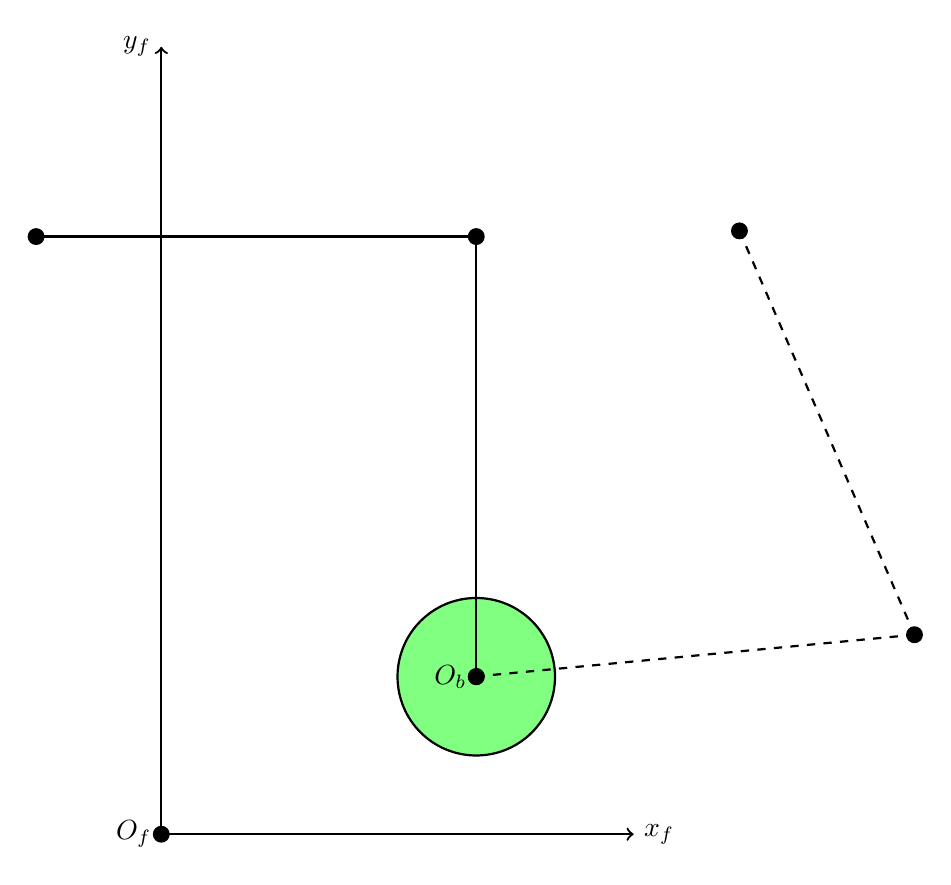
\begin{tikzpicture}

  \def\lone{5.59} 
  \def\ltwo{5.59}

  \def\thetazero{90}
  \def\thetaone{0}
  \def\thetatwo{90} 

  \coordinate (O) at (0,0);
  \coordinate (Ob) at (4,2);
  \coordinate (A) at ({4+\lone*cos(\thetaone+\thetazero)},{2+\lone*sin(\thetaone+\thetazero)});
  \coordinate (B) at ({4+\lone*cos(\thetaone+\thetazero) + \ltwo*cos(\thetaone + \thetatwo+\thetazero)}, 
                      {2+\lone*sin(\thetaone+\thetazero) + \ltwo*sin(\thetaone + \thetatwo+\thetazero)});
  \coordinate (Obp) at (4.00068, 2.00333);
  \coordinate (Ap) at (9.56548, 2.53356);
  \coordinate (Bp) at (7.34235, 7.66248);

  \draw[dashed,fill=green!25] (Obp) circle (1);
  \draw[thick,fill=green!50] (Ob) circle (1);

  \draw[thick, black] (Ob) -- (A);
  \draw[thick, black] (A) -- (B);
  \draw[thick, black, dashed] (Obp) -- (Ap);
  \draw[thick, black, dashed] (Ap) -- (Bp);

  \draw[thick,black,->] (O) -- (0,10) node[anchor=east]{$y_f$};
  \draw[thick,black,->] (O) -- (6,0) node[anchor=west]{$x_f$};

  \filldraw[fill=black] (O) circle (0.1);
  \filldraw[fill=black] (Ob) circle (0.1);
  \filldraw[fill=black] (A) circle (0.1);
  \filldraw[fill=black] (B) circle (0.1);
  \filldraw[fill=black] (Obp) circle (0.1);
  \filldraw[fill=black] (Ap) circle (0.1);
  \filldraw[fill=black] (Bp) circle (0.1);

  \node[anchor=east] at (O) {$O_f$};
  \node[anchor=east] at (Ob) {$O_b$};

\end{tikzpicture}}}}
              \subfloat[][\emph{Simulation 2.}]
                {\scalebox{0.5}{\scalebox{0.8}{
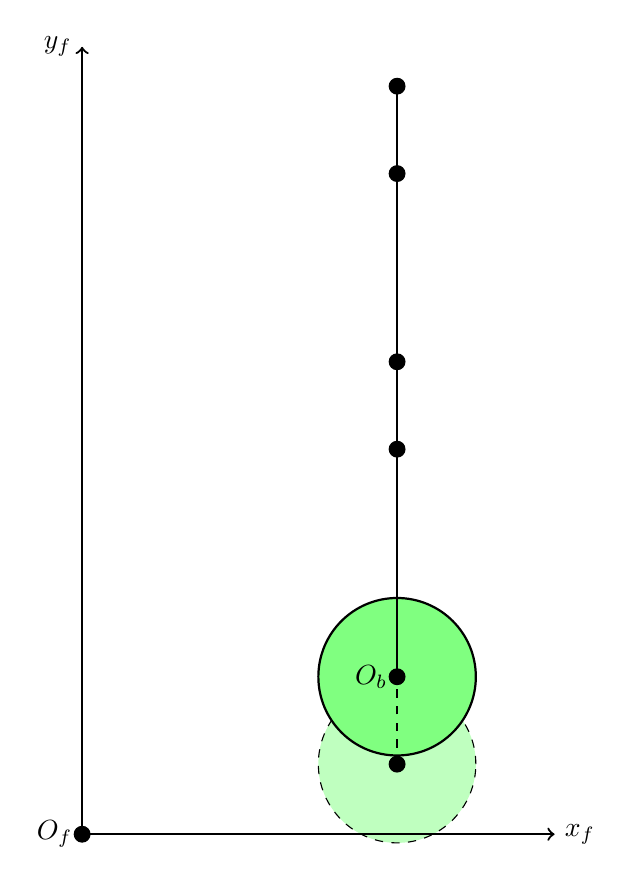
\begin{tikzpicture}

  \def\lone{4} 
  \def\ltwo{3.5}

  \def\thetazero{90}
  \def\thetaone{0}
  \def\thetatwo{0} 

  \coordinate (O) at (0,0);
  \coordinate (Ob) at (4,2);
  \coordinate (A) at ({4+\lone*cos(\thetaone+\thetazero)},{2+\lone*sin(\thetaone+\thetazero)});
  \coordinate (B) at ({4+\lone*cos(\thetaone+\thetazero) + \ltwo*cos(\thetaone + \thetatwo+\thetazero)}, 
                      {2+\lone*sin(\thetaone+\thetazero) + \ltwo*sin(\thetaone + \thetatwo+\thetazero)});
  \coordinate (Obp) at (4,0.89);
  \coordinate (Ap) at (4,4.89);
  \coordinate (Bp) at (4,8.39);

  \draw[dashed,fill=green!25] (Obp) circle (1);
  \draw[thick,fill=green!50] (Ob) circle (1);

  \draw[thick, black] (Ob) -- (A);
  \draw[thick, black] (A) -- (B);
  \draw[thick, black, dashed] (Obp) -- (Ap);
  \draw[thick, black, dashed] (Ap) -- (Bp);

  \draw[thick,black,->] (O) -- (0,10) node[anchor=east]{$y_f$};
  \draw[thick,black,->] (O) -- (6,0) node[anchor=west]{$x_f$};

  \filldraw[fill=black] (O) circle (0.1);
  \filldraw[fill=black] (Ob) circle (0.1);
  \filldraw[fill=black] (A) circle (0.1);
  \filldraw[fill=black] (B) circle (0.1);
  \filldraw[fill=black] (Obp) circle (0.1);
  \filldraw[fill=black] (Ap) circle (0.1);
  \filldraw[fill=black] (Bp) circle (0.1);

  \node[anchor=east] at (O) {$O_f$};
  \node[anchor=east] at (Ob) {$O_b$};

\end{tikzpicture}}}}
                \caption{Initial and final (dashed) position of the VMS after the impact for the two different simulations, ten seconds long.}
              \end{figure}
        \end{column}
    \end{columns}
\end{frame}

\begin{frame}{Rigid Bodies}
    \begin{figure}
        \centering
        \subfloat
        {\includesvg[scale=0.2]{../../Images/free_motion_x.svg}} \quad
      \subfloat
        {\includesvg[scale=0.2]{../../Images/free_motion_y.svg}} \quad
        \subfloat
        {\includesvg[scale=0.2]{../../Images/free_motion_theta.svg}} \\
        \subfloat
        {\includesvg[scale=0.2]{../../Images/free_motion_q1.svg}} \quad
        \subfloat
        {\includesvg[scale=0.2]{../../Images/free_motion_q2.svg}}
        \caption{VMS generalized coordinates' displacement after the catching of the payload when no control is performed, Simulation~1.}
      \end{figure}
\end{frame}

\begin{frame}{Rigid Bodies}
    \begin{figure}
        \centering
        \subfloat
        {\includesvg[scale=0.2]{../../Images/free_motion_x2.svg}} \quad
      \subfloat
        {\includesvg[scale=0.2]{../../Images/free_motion_y2.svg}} \quad
        \subfloat
        {\includesvg[scale=0.2]{../../Images/free_motion_theta2.svg}} \\
        \subfloat
        {\includesvg[scale=0.2]{../../Images/free_motion_q12.svg}} \quad
        \subfloat
        {\includesvg[scale=0.2]{../../Images/free_motion_q22.svg}}
        \caption{VMS generalized coordinates' displacement after the catching of the payload when no control is performed, Simulation~2.}
      \end{figure}
\end{frame}

\begin{frame}{Rigid Bodies}
  \begin{itemize}
    \item Controlled motion:
    \begin{equation}
      \begin{bmatrix}
        M'_{tt}&M'_{tr}\\
        M'_{rt}&M'_{rr}
      \end{bmatrix}
      \begin{bmatrix}
        \ddot{p}_t\\
        \ddot{p}_r
      \end{bmatrix}+\begin{bmatrix}
        C'_{t}\\
        C'_{r}
      \end{bmatrix}=\begin{bmatrix}
        \textbf{0}\\
          u
        \end{bmatrix}
    \end{equation}
    \item Translational coordinates as a function of rotational ones:
    \begin{equation}
      \ddot{p}_t=-{M'}_{tt}^{-1}(M'_{tr}\ddot{p}_r+C'_t)
    \end{equation}
    \item Final equation:
    \begin{equation}
      \ddot{p}_r\tilde{M}+\tilde{C}=u
    \end{equation}
    \item Feedback linearization:
    \begin{equation}
      u=\hat{M}[\ddot{q}_d+K_d(\dot{q}_d-\dot{q})+K_p(q_d-q)]+\hat{C}
    \end{equation}
  \end{itemize}
\end{frame}

\begin{frame}{Rigid Bodies}
  \begin{itemize}
    \item If $\hat{M}\approx \tilde{M}$ and $\hat{C}\approx\tilde{C}$:
    \begin{equation}
      \ddot{e}+K_d\dot{e}+K_pe=0
    \end{equation}
    \begin{itemize}
      \item decoupled;
      \item linear;
      \item $\omega_n=\sqrt{K_{p_i}}$ and $\xi=\frac{K_{d_i}}{2\sqrt{K_{p_i}}}$.
    \end{itemize}
    \item Critically damped when
    \begin{equation}
     \xi=1 \quad \Rightarrow \quad K_d=2\sqrt{K_p}
    \end{equation}
  \end{itemize}
\end{frame}

\begin{frame}{Rigid Bodies}
  \begin{figure}
      \centering
      \subfloat
      {\includesvg[scale=0.2]{../../Images/controlled_motion_x.svg}} \quad
    \subfloat
      {\includesvg[scale=0.2]{../../Images/controlled_motion_y.svg}} \quad
      \subfloat
      {\includesvg[scale=0.2]{../../Images/controlled_motion_theta.svg}} \\
      \subfloat
      {\includesvg[scale=0.2]{../../Images/controlled_motion_q1.svg}} \quad
      \subfloat
      {\includesvg[scale=0.2]{../../Images/controlled_motion_q2.svg}}
      \caption{VMS generalized coordinates' displacement after the catching of the payload when control is performed, Simulation~1. In yellow, an underdamped behaviour ($\xi=0.5$), in blue a critically damped behaviour ($\xi=1$), in green an overdamped behaviour ($\xi=1.5$).}
    \end{figure}
\end{frame}

\begin{frame}{Rigid Bodies}
  \begin{figure}
      \centering
      \subfloat
      {\includesvg[scale=0.2]{../../Images/controlled_motion_x2.svg}} \quad
    \subfloat
      {\includesvg[scale=0.2]{../../Images/controlled_motion_y2.svg}} \quad
      \subfloat
      {\includesvg[scale=0.2]{../../Images/controlled_motion_theta2.svg}} \\
      \subfloat
      {\includesvg[scale=0.2]{../../Images/controlled_motion_q12.svg}} \quad
      \subfloat
      {\includesvg[scale=0.2]{../../Images/controlled_motion_q22.svg}}
      \caption{VMS generalized coordinates' displacement after the catching of the payload when control is performed, Simulation~2. In yellow, an underdamped behaviour ($\xi=0.5$), in blue a critically damped behaviour ($\xi=1$), in green an overdamped behaviour ($\xi=1.5$).}
    \end{figure}
\end{frame}

\begin{frame}{Elastic Bodies}
  \begin{itemize}
    \item Arms modeled ad Euler-Bernoulli Beams:
    \begin{equation}
      \begin{array}{c}
      w(x,t)=\sum_{n=1}^\infty W_n(x)Q_n(t)\\
      Q(t)=A\cos{\omega t}+B\sin{\omega t}\\
      W(x)=c_1\cos(\beta x)+c_2\sin{\beta x}+c_3\cosh{\beta x}+c_4\sinh{\beta x}
      \end{array}
    \end{equation}
    \item Elasticity Matrix~\cite{elasticity}:
    \begin{equation}
      \prescript{i}{i+1}{E}=\begin{bmatrix}
        1&0&0&0\\
        0&1&0&W_i(x)Q_i(t)\\
        0&0&1&0
      \end{bmatrix}
    \end{equation}
    \item The number of coordinates increases: $p=\{x_b,y_b,\theta_b,q_1,q_2,Q_1,Q_2\}$.
  \end{itemize}
\end{frame}

\begin{frame}{Elastic Bodies}
  \begin{itemize}
    \item Elastic potential energy: 
    \begin{equation}
      \begin{split}
      U&=\frac{1}{2}\int_{0}^{l_i}ES\Big(\frac{\partial^2 w(x,t)}{\partial x^2}\Big)^2\,dx\\
       &=\frac{1}{2}\int_{0}^{l_i}ES\Big(\frac{\partial^2 W(x)}{\partial x^2}Q(t)\Big)^2\,dx
      \end{split}
    \end{equation}
    \item Included in the stiffness matrix:
    \begin{equation}
      \begin{array}{c}
        \frac{d}{dt}\frac{\partial U}{\partial \dot{Q}_i}-\frac{\partial U}{\partial Q_i}=0+\int_{0}^{l_i}ES\frac{\partial^2 W(x)}{\partial x^2}\,dx\\
        M\ddot{p}+C+Kp=u+J^Tf_I\\
        K_i=\int_{0}^{l_i}E_iS_i\frac{\partial^2 W_i(x)}{\partial x^2}\,dx
      \end{array}
    \end{equation}
  \end{itemize}
\end{frame}

\begin{frame}{Elastic Bodies}
  \begin{figure}
      \centering
      \subfloat
      {\includesvg[scale=0.2]{../../Images/elastic_controlled_x.svg}} \quad
    \subfloat
      {\includesvg[scale=0.2]{../../Images/elastic_controlled_y.svg}} \quad
      \subfloat
      {\includesvg[scale=0.2]{../../Images/elastic_controlled_q1.svg}} \\
      \subfloat
      {\includesvg[scale=0.2]{../../Images/elastic_controlled_q2.svg}} \quad
      \subfloat
      {\includesvg[scale=0.2]{../../Images/elastic_controlled_QQ1.svg}} \quad
      \subfloat
      {\includesvg[scale=0.2]{../../Images/elastic_controlled_QQ2.svg}} 
      \caption{VMS generalized coordinates’ displacement after the catching of the payload when control is performed, Simulation~1. Arms modeled as Euler-Bernoulli beams.}
    \end{figure}
\end{frame}

\begin{frame}{Elastic Bodies}
  \begin{figure}
      \centering
      \subfloat
      {\includesvg[scale=0.2]{../../Images/elastic_controlled_x2.svg}} \quad
    \subfloat
      {\includesvg[scale=0.2]{../../Images/elastic_controlled_y2.svg}} \quad
      \subfloat
      {\includesvg[scale=0.2]{../../Images/elastic_controlled_q12.svg}} \\
      \subfloat
      {\includesvg[scale=0.2]{../../Images/elastic_controlled_q22.svg}} \quad
      \subfloat
      {\includesvg[scale=0.2]{../../Images/elastic_controlled_QQ12.svg}} \quad
      \subfloat
      {\includesvg[scale=0.2]{../../Images/elastic_controlled_QQ22.svg}} 
      \caption{VMS generalized coordinates’ displacement after the catching of the payload when control is performed, Simulation~2. Arms modeled as Euler-Bernoulli beams.}
    \end{figure}
\end{frame}

\section{Mass and Velocity Retrieval}

\begin{frame}{Linearization}
  \begin{itemize}
    \item Approximations:
    \begin{itemize}
      \item No spacecraft translation;
      \item No spacecraft rotation;
      \item Linearization around equilibrium position.
    \end{itemize}
    \item First-order Taylor expansion:
    \begin{equation}
      D(\textbf{x})=D(q_1,q_2,\dot{q}_1,\dot{q}_2,\ddot{q}_1,\ddot{q}_2)=M'(q_1,q_2)\begin{bmatrix}
        \ddot{q}_1\\
        \ddot{q}_2
      \end{bmatrix}+C'(q_1,q_2,\dot{q}_1,\dot{q}_2)
    \end{equation}
    \begin{equation}
      D(\textbf{x})\approx D(\bar{\textbf{x}})+(\textbf{x}-\bar{\textbf{x}})^T\nabla T(\textbf{x})
    \end{equation}
    \item New linearized dynamics:
    \begin{equation}
      M_{lin}\ddot{q}+C_{lin}\dot{q}+K_{lin}q-\delta=0
    \end{equation}
  \end{itemize}
\end{frame}

\begin{frame}{Joints' Decoupling}
  \begin{itemize}
    \item Displacement of one arm neglgible for the displacement of the other one (true when $\hat{M}=M'$).
    \item New equations:
    \begin{equation}
      \begin{array}{l}
        \ddot{q}_1+\frac{\hat{m_1}}{\tilde{m}_1}k_d\dot{e}_1+\frac{\hat{m_1}}{\tilde{m}_1}k_p e_1=0\\
        \ddot{q}_2+\frac{\hat{m_2}}{\tilde{m}_2}k_d\dot{e}_2+\frac{\hat{m_2}}{\tilde{m}_2}k_p e_2=0
      \end{array}
    \end{equation}
    \item Damping coefficient:
    \begin{equation}
      \xi'=\frac{\hat{m}k_v}{2\omega_n \tilde{m}}=\frac{\hat{m}2\sqrt{k_p}}{2\sqrt{\frac{\hat{m}}{\tilde{m}}k_p} \tilde{m}}=\sqrt{\frac{\hat{m}}{\tilde{m}}}
      \label{mass_relation}
    \end{equation}
  \end{itemize}
\end{frame}

\begin{frame}{Joints' Decoupling}
  \begin{columns}
    \begin{column}{0.5\textwidth}
      \begin{itemize}
        \item Position Roots: find overshoot, find parametrix solution of equation and solve: $q(t^*,\tilde{m})=q^*$.
        \item Mass Fit: minimize error with non-linear regression, parameter is the mass. We can add noise:
        \vspace{2mm}
        \begin{figure}
          \centering
          \includesvg[scale=0.11]{../../Images/noisy_data.svg}
          \caption{Noisy data to simulate a real scenario in orange.}
        \end{figure}
      \end{itemize}
    \end{column}
    \begin{column}{0.5\textwidth}
      \begin{figure}
        \centering
        \includesvg[scale=0.2]{../../Images/parametric_plot.svg}
        \caption{Parametric plot of the first joint's time evolution, first simulation. The real mass is $\SI{3000}{\kilogram}$.}
      \end{figure}
    \end{column}
  \end{columns}
\end{frame}

\begin{frame}{Joints' Decoupling}
  \begin{itemize}
    \item Derivative Roots:
    \begin{equation}
      \begin{array}{c}
        \tilde{m}\ddot{q}+\hat{m}k_d\dot{q}+\hat{m}k_p (q-q_d)=0\\
        \tilde{m}\ddot{q}+\hat{m}k_d\dot{q}+\hat{m}k_p q=\hat{m}k_pq_d\\
        q(t)=q_d\Big[1-\frac{e^{-\xi\omega_nt}}{\sqrt{1-\xi^2}}\sin{(\omega_dt+\theta)}\Big]+\Big[q_0\cos{(\omega_d)t}+\frac{\dot{q}_0+\xi\omega_n q_0}{\omega_d}\sin{(\omega_dt)}\Big]e^{-\xi \omega_n t}\\
        \tan{(\sqrt{1-\xi^2}\omega_nt^*)}=\beta(\xi)
      \end{array}
    \end{equation}
    \item Damping coefficient and natural frequency fit: non-linear regression of closed-form solution, parameters are $\xi$ and $\omega_n$.
  \end{itemize}
\end{frame}

\begin{frame}{Coupled Solution}
  \begin{columns}
    \begin{column}{0.5\textwidth}
      \begin{itemize}
        \item Continous Domain: solve coupled equations with Wolfram's \texttt{ParametricNDSolve} $\rightarrow q(m,t)$:
        \begin{equation}
          \begin{array}{c}
            \Gamma(m)=\int_{0}^{T}\Big[q(m,t)-q_{data}(t)\Big]^2\\
            m^*=\min_{m}\Gamma(m)
          \end{array}
        \end{equation}
        \item Discrete Domain: equations solved with Maple, closed-form solution:
        \begin{equation}
          \varGamma(m)=\sum_{k=0}^{N_p}\Big[q(m,\frac{T}{N_p}k)-q_{data}(\frac{T}{N_p}k)\Big]^2
        \end{equation}
      \end{itemize}
    \end{column}
    \begin{column}{0.5\textwidth}
      \begin{figure}
        \centering
        \includesvg[scale=0.15]{../../Images/discrete_25p.svg}
        \caption{In blue is the continous solution, in red is the discretized one.}
      \end{figure}
    \end{column}
  \end{columns}
\end{frame}

\begin{frame}{Velocity Extraction}
  \begin{itemize}
    \item From final velocities relation:
    \begin{equation}
      \dot{p}_f=G^{-1}H
    \end{equation}
    we can write:
    \begin{equation}
      \begin{array}{l}
        H=G\dot{p}_f\\
        \Rightarrow M\dot{p}_i+J^T(J_O^+)^TM_O\dot{\psi}_i=G\dot{p}_f\\
        \Rightarrow \dot{\psi}_i=M_O^{-1}J_O^T(J^+)^T(G\dot{p}_f-M\dot{p}_i)
      \end{array}
    \end{equation}
    \item Good results for translational velocities, big numerical erros for $\dot{\theta}_O$.
    \item Previous assumption: docking ($\dot{\theta}_O\approx 0$).
  \end{itemize}
\end{frame}

\section{Results}

\begin{frame}{Mass Extraction}
  \begin{figure}
    \centering
    \subfloat[]{\includesvg[scale=0.16]{../../Images/masses0_1.svg}} \quad
    \subfloat[]{\includesvg[scale=0.16]{../../Images/massespi6_1.svg}}
    \caption{Joints' Decoupling.}
  \end{figure}
\end{frame}

\begin{frame}{Mass Extraction}
  \begin{figure}
    \centering
    \subfloat[]{\includesvg[scale=0.16]{../../Images/massespi3_1.svg}} \quad
    \subfloat[]{\includesvg[scale=0.16]{../../Images/massespi2_1.svg}}
    \caption{Joints' Decoupling.}
  \end{figure}
\end{frame}

\begin{frame}{Mass Extraction}
  \begin{figure}
    \centering
    \subfloat[]{\includesvg[scale=0.16]{../../Images/masses_uncoupled_1.svg}} \quad
    \subfloat[]{\includesvg[scale=0.16]{../../Images/masses_uncoupled_1.svg}}
    \caption{Coupled Solution.}
  \end{figure}
\end{frame}

\begin{frame}{Velocity Extraction}
  \begin{figure}
    \centering
    \subfloat[]{\includesvg[scale=0.16]{../../Images/velpi2_1.svg}} \quad
    \subfloat[]{\includesvg[scale=0.16]{../../Images/velpi6_1.svg}}
    \caption{Velocity error for Simulation~1.}
  \end{figure}
\end{frame}

\begin{frame}{Velocity Extraction}
  \begin{figure}
    \centering
    \subfloat[]{\includesvg[scale=0.16]{../../Images/velpi2_2.svg}} \quad
    \subfloat[]{\includesvg[scale=0.16]{../../Images/velpi6_2.svg}}
    \caption{Velocity error for Simulation~2.}
  \end{figure}
\end{frame}

\begin{frame}{Conclusion}
  \begin{itemize}
    \item Joints' Decoupling:
    \begin{itemize}
      \item Pro: simple closed-form equation
      \item Cons: depend significantly on VMS configuration.
      \item $\xi$ and $\omega_n$ fit best one.
      \item When $\hat{m}>m$ better results: displacement is smaller, linerization error reduced.
    \end{itemize}
    \item Coupled Solution:
    \begin{itemize}
      \item Pro: less susceptible to VMS configuration.
      \item Cons: require more computational power (continuous method).
      \item Discrete method is faster ($\approx \SI{0.03}{\second}$ vs $\SI{1.5}{\second}$)
    \end{itemize}
  \end{itemize}
\end{frame}

\bibliographpage

\backmatter

\section{Q\&A}

\begin{frame}{Elastic Vibrations}
  \begin{figure}
    \centering
    \subfloat[\emph{First joint.}]{\includesvg[scale=0.3]{../../Images/beat_1.svg}}\quad
    \subfloat[\emph{Second joint.}]{\includesvg[scale=0.3]{../../Images/beat_2.svg}}
    \caption{Extended temporal window of joints' elastic coordinates for Simulation 1. The oscillations change in time due to the movement of the arms.}
  \end{figure}
\end{frame}

\begin{frame}{Elastic Vibrations}
  \begin{figure}
    \centering
    \subfloat[\emph{First joint.}]{\includesvg[scale=0.3]{../../Images/no_beat_1.svg}}\quad
    \subfloat[\emph{Second joint.}]{\includesvg[scale=0.3]{../../Images/no_beat_2.svg}}
    \caption{Extended temporal window of joints' elastic coordinates for Simulation 1. The oscillations are constant since the arms do not move after the impact.}
  \end{figure}
\end{frame}